\section{Results}
We first explore the differences between learning directly on a target task and first learning on source task (i.e. using our transfer learning algorithm), using the metrics that we defined in Section~\ref{sub:tl_metrics}. For the regular algorithm, we use the \textit{REINFORCE} that was discussed in Section~\ref{sub:rl_policy_gradient}. The learning curve of both algorithms on the target task is visualized in Figure~\ref{fig:tla_re_5envs}.
\begin{figure}[H]
    \centering
    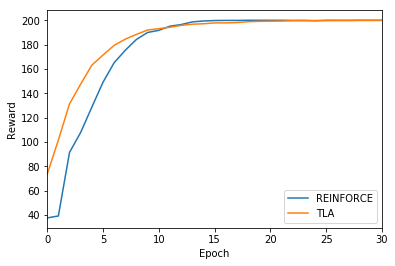
\includegraphics[width=.8\linewidth]{images/tla_re_target_5envs.png}
    \caption[Learning curves for \textit{REINFORCE} and \textit{TLA}]{Learning curves of the \textit{REINFORCE} algorithm and our transfer learning algorithm (\textit{TLA}). The learning curves are only showed until epoch 30 in order to better show the initial performance of both algorithms. Both algorithms were converged and achieved the same rewards after epoch 30.}
    \label{fig:tla_re_5envs}
\end{figure}
It can be seen that, on average, the jumpstart performance of our algorithm is higher than when we do not use transfer learning.
%statistical test?
Specifically, the mean jumpstart performance for \textit{REINFORCE} is $37.575$, while the jumpstart performance for our algorithm is $73.414$.\\
Both algorithms eventually reach the maximum reward ($200$) and as such they have the same asymptotic performance.\\

To further explore the jumpstart performance, we will look at boxplots of the jumpstarts of both algorithms, computed using all the 100 runs of both algorithms. These are shown in Figure~\ref{fig:boxplot_tla_re_5envs}.
\begin{figure}[H]
    \centering
    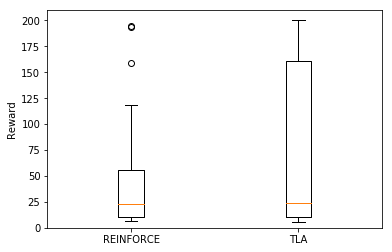
\includegraphics[width=.8\linewidth]{images/boxplot_tla_re_target_5envs.png}
    \caption{Boxplot of the jumpstart performance of \textit{REINFORCE} and our transfer learning algorithm (\textit{TLA}).}
    \label{fig:boxplot_tla_re_5envs}
\end{figure}
We can see that, although the mean jumpstart performances are different, there is little difference between the medians: $22.774$ for \textit{REINFORCE} and $23.459$ for our algorithm. However, our algorithm is able to reach a higher initial performance more often. In 75\% of the cases, the jumpstart performance for \textit{REINFORCE} is below $55.535$, while it is $160.595$ for our algorithm.
